\section{Component design}\label{sec:components}

This section describes each component: its responsibility, its inputs and outputs, and the main design decisions. Section~\ref{sec:examples} then shows the components working together on concrete scenarios.

%-----------------------------------------------------------------
\subsection{Principal authentication and binding}

\textbf{Responsibility:} make sure that every task is launched by a known, authenticated person, and record who that person is.

We reuse the university's existing OpenID Connect (OIDC) provider rather than building our own identity verification. From the terminal, the principal runs a small helper (\code{kya login}) that performs the OAuth~2.0 device authorization flow (RFC~8628): it prints a short code, the principal confirms it in a browser, and the helper stores an ID token locally. A thin wrapper adds this token as gRPC metadata to every \code{ax} call:

\begin{lstlisting}[language=bash]
kya login                                  # once per day; opens university SSO
ax --server kya-admission.kya-system:8080 apply -f task.yaml
\end{lstlisting}

The admission proxy validates the token (signature, issuer, audience, expiry) and extracts the principal's stable identifier (\code{sub}), e-mail and group memberships. These become the \code{principal} block of the passport. For the demo we also support a local development identity provider (e.g.\ Keycloak or Dex) so the system can run without university infrastructure.

\begin{keyidea}[Why OIDC is enough for principal binding here]
KYA products in the finance sector bind agents to people through full identity verification (documents, face match). In a university or company setting, the organisation has already verified its members; OIDC login inherits that verification. The design keeps the principal block generic, so a stronger identity source can be plugged in later.
\end{keyidea}

%-----------------------------------------------------------------
\subsection{Policy model}

\textbf{Responsibility:} describe, per group of principals, which tasks may run and what they may do. Policies are written by platform operators as YAML documents of our own kind \code{AgentPolicy}, stored in the policy store (PostgreSQL) and applied with \code{kya policy apply}.

\begin{lstlisting}[language=yaml,caption={An \code{AgentPolicy} for students building shopping agents.},label={lst:policy}]
apiVersion: kya.io/v1alpha1
kind: AgentPolicy
metadata:
  name: students-shopping
spec:
  principals:
    groups: ["hacettepe-cs/design-team"]
  images:
    allow: ["ghcr.io/example/shopping-agent@sha256:*"]  # pinned digests only
  models:
    allow: ["anthropic/claude-*", "google/gemini-*"]
  passport:
    ttl: 2h                   # passports expire quickly
    maxDelegationDepth: 2     # task -> sub-task -> sub-sub-task
  visa:                       # the widest visa this group can ever get
    hosts: ["shop.example.com", "api.llm.example"]
    actions:
      - name: catalog.read
      - name: order.create
        limits:
          perRequest: { value: 500,  currency: TRY }
          total:      { value: 1000, currency: TRY }
        approvalAbove: { value: 300, currency: TRY }
  trust:
    stepUpBelow: 0.6
    suspendBelow: 0.4
\end{lstlisting}

A task may ask for \emph{less} than the policy allows by including an environment entry named \code{KYA\_\allowbreak{}REQUESTED\_\allowbreak{}VISA} (JSON) in its \code{spec.env}. Because the environment is part of the task manifest, the request is covered by the manifest hash in the passport. The effective visa is the intersection of the policy visa and the requested visa. (If AX later adds annotations to task metadata, the request can move there.)

\textbf{Actions} are names chosen by relying parties (\code{order.create}, \code{payments.pay}, \ldots). A relying party publishes which HTTP routes correspond to which action names; the verifier SDK maps routes to actions (Section~\ref{sec:verifier}). The gateway only knows hosts; actions and amounts are enforced by the verifier, which sees the application-level meaning of a request.

%-----------------------------------------------------------------
\subsection{Admission proxy}

\textbf{Responsibility:} be the only entry point to \code{ax-server}; authenticate, check policy, request a passport, adjust the task, and forward it.

The admission proxy is a Go service that implements the \code{ax.v1alpha1.AX} gRPC service using the generated types from \codeurl{github.com/google/ax/pkg/apis/v1alpha1}. Read-only calls (\code{GetTask}, \code{ListTasks}, \code{WatchTask}) are forwarded after authentication, filtered so that principals only see their own tasks. \code{CreateTask} goes through the following pipeline:

\begin{enumerate}
  \item \textbf{Authenticate} the ID token; reject with \code{UNAUTHENTICATED} if missing or invalid.
  \item \textbf{Find the applicable policy} by the principal's groups.
  \item \textbf{Validate} the image (must be a pinned digest matching \code{images.allow}), the model, resource limits and the requested visa. Reject with \code{PERMISSION\_DENIED} and a human-readable reason otherwise, e.g.\ \emph{``image tag :latest is not allowed; pin a digest''}.
  \item \textbf{Compute the manifest hash}: SHA-256 over a canonical serialisation of the task spec and its bound workspaces. Any change to the task (command, environment, repositories) changes the hash and therefore the passport.
  \item \textbf{Request a passport} from the passport authority with task identity, principal, effective visa and TTL.
  \item \textbf{Adjust the task}: set \code{spec.image} to the KYA runner variant of the requested image (a thin layer on top that replaces \codeurl{/usr/local/bin/ax-task-runner}); add environment entries \code{HTTPS\_PROXY}, \code{HTTP\_PROXY} (with a per-task proxy credential), \code{KYA\_PASSPORT\_ID} and \code{KYA\_EVENTS\_URL}.
  \item \textbf{Forward} the call to \code{ax-server}, record \code{task.created} and \code{passport.issued} in the audit ledger, and return AX's response unchanged.
\end{enumerate}

\begin{example}[A rejected launch]
A student applies a task whose image is \code{ghcr.io/example/shopping-agent:latest} and whose requested visa includes \code{payments.pay}. The proxy answers:
\begin{lstlisting}[language={}]
Error: PERMISSION_DENIED: task "shop-8b21" rejected by policy students-shopping:
  - image must be pinned by digest (got tag "latest")
  - action "payments.pay" is not allowed for group hacettepe-cs/design-team
\end{lstlisting}
Nothing reaches AX, and the rejection is logged with the principal's identity.
\end{example}

%-----------------------------------------------------------------
\subsection{Passport authority}

\textbf{Responsibility:} issue, store, publish and revoke passports; hold the issuer signing key; publish public keys and revocation status.

\subsubsection{Passport content}

A passport is a JSON Web Token signed by the PA with Ed25519 (JWS algorithm \code{EdDSA}). Figure~\ref{fig:passport} shows its four parts; Listing~\ref{lst:passport} shows the full claim set.

\begin{figure}[H]
  \centering
  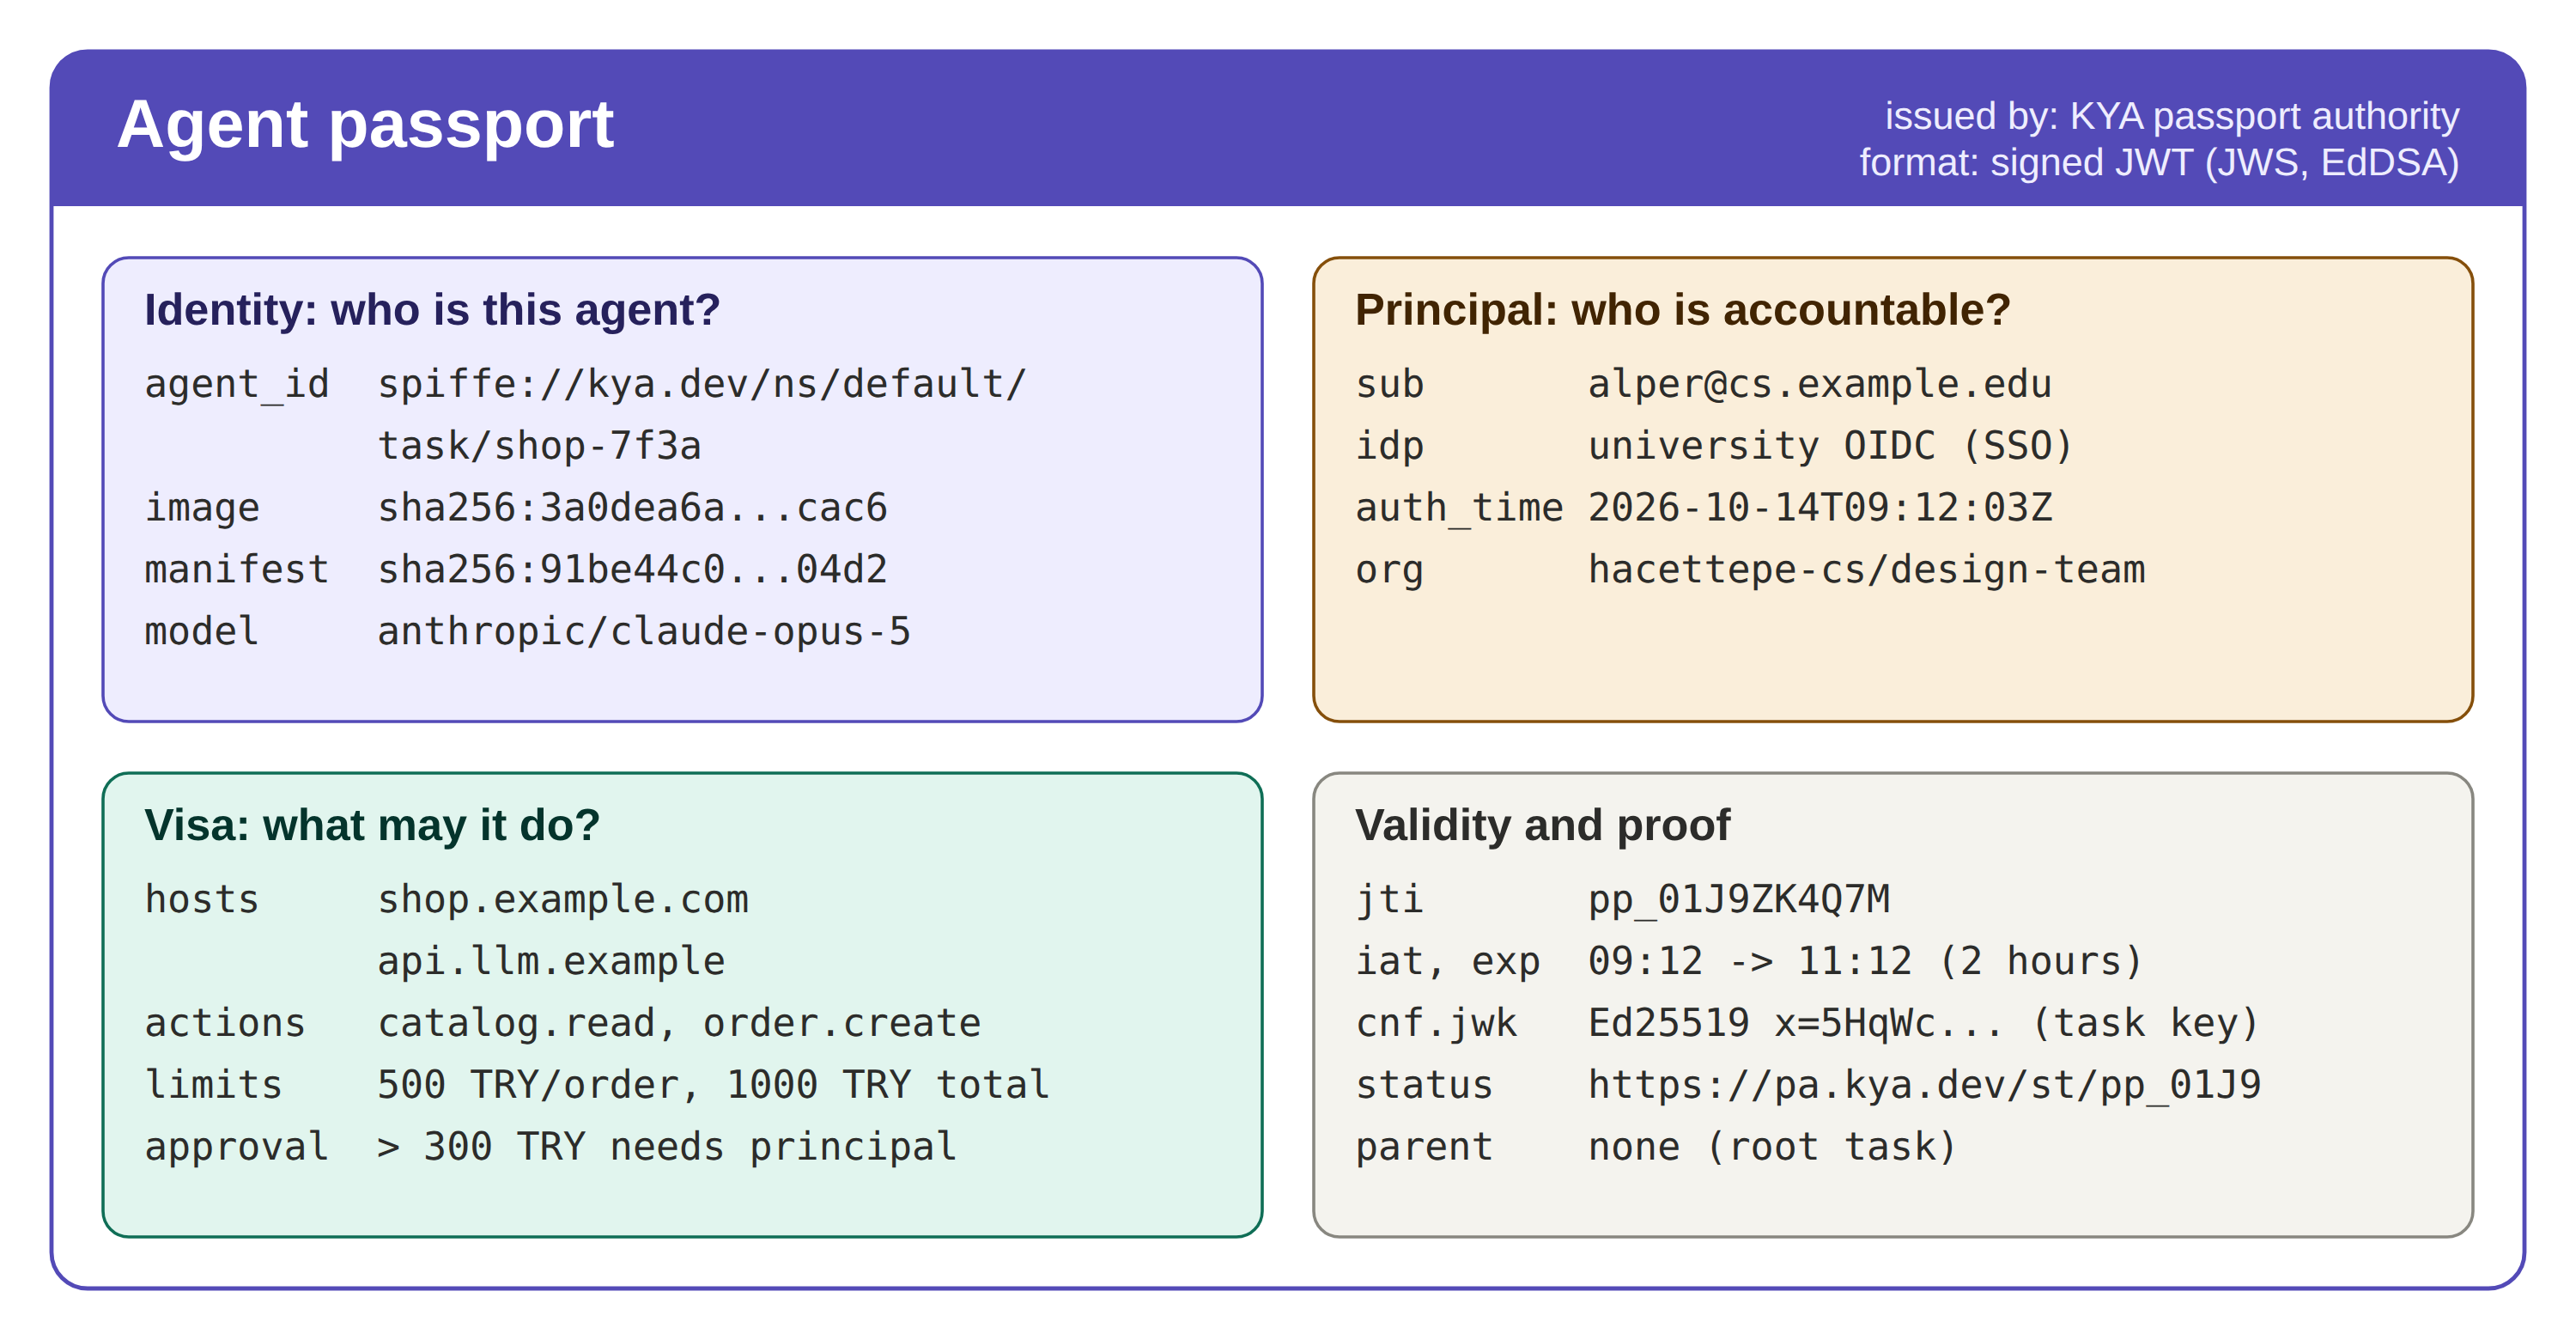
\includegraphics[width=0.92\linewidth]{passport.png}
  \caption{Anatomy of an agent passport. Each quadrant corresponds to one question a relying party may ask.}
  \label{fig:passport}
\end{figure}

\begin{lstlisting}[language=json,caption={Decoded payload of the passport in Figure~\ref{fig:passport}.},label={lst:passport}]
{
  "iss": "https://pa.kya.dev",
  "sub": "spiffe://kya.dev/ns/default/task/shop-7f3a",
  "aud": "kya:relying-parties",
  "jti": "pp_01J9ZK4Q7M",
  "iat": 1760433123,  "nbf": 1760433123,  "exp": 1760440323,
  "cnf": { "jwk": { "kty": "OKP", "crv": "Ed25519", "x": "5HqWc...", "kid": "k-7f3a" } },
  "kya": {
    "ver": "0.1",
    "task": {
      "atespace": "default", "name": "shop-7f3a",
      "image": "sha256:3a0dea6a...cac6", "manifest": "sha256:91be44c0...04d2",
      "model": "anthropic/claude-opus-5"
    },
    "principal": {
      "sub": "alper@cs.example.edu", "idp": "https://sso.example.edu",
      "auth_time": 1760432523, "org": "hacettepe-cs/design-team"
    },
    "visa": {
      "hosts": ["shop.example.com", "api.llm.example"],
      "actions": [
        { "name": "catalog.read" },
        { "name": "order.create",
          "per_request": { "value": 500,  "currency": "TRY" },
          "total":       { "value": 1000, "currency": "TRY" },
          "approval_above": { "value": 300, "currency": "TRY" } }
      ]
    },
    "parent": null,
    "status": "https://pa.kya.dev/status/pp_01J9ZK4Q7M"
  }
}
\end{lstlisting}

\textbf{The agent identifier} follows the SPIFFE format (\codeurl{spiffe://<trust-domain>/ns/<atespace>/task/<name>}), so that when AX ships native SPIFFE identities for tasks~\cite{ax-roadmap} the two can be aligned.

\textbf{Privacy.} The passport reveals the principal to every relying party. For services that do not need to know who the person is, the PA can issue a \emph{pairwise pseudonymous} principal identifier (a hash of the principal and the relying party's host) while keeping the real mapping in the audit ledger for investigations.

\subsubsection{Keys and proof of possession}

There are two kinds of keys:

\begin{itemize}
  \item The \textbf{issuer key} of the PA signs passports. Its public half is published at \codeurl{https://pa.kya.dev/.well-known/jwks.json}. It is rotated monthly; old keys stay published until all passports they signed have expired.
  \item A \textbf{task key} is generated by the PA for each task (Ed25519). Its public half is embedded in the passport's \code{cnf.jwk} claim (RFC~7800). Its private half is handed to the egress gateway over mutual TLS and is kept only in the gateway's memory; the PA does not retain it, and it never enters the sandbox.
\end{itemize}

Because the passport names the key that must sign each request, a passport copied from a log file or network capture is useless on its own: whoever presents it must also produce a fresh signature with the task key.

\subsubsection{Revocation}

Passports are short-lived (two hours by default), which limits the damage of any mistake. For faster reaction, the PA supports explicit revocation:

\begin{itemize}
  \item \code{POST /v1/passports/\{jti\}:revoke} (used by the trust observer and the console);
  \item a per-passport status URL (\code{status} claim) returning \code{active}, \code{suspended} or \code{revoked};
  \item a signed \textbf{revocation list} of recently revoked \code{jti} values at \code{/v1/revocations}, which verifiers poll every 30~seconds or receive through a server-sent event stream. This keeps per-request verification local (NFR4) while bounding the revocation delay.
\end{itemize}

\subsubsection{PA API sketch}

\begin{center}
\small
\begin{tabularx}{\linewidth}{@{}L{5.7cm}Y@{}}
\toprule
\textbf{Endpoint} & \textbf{Purpose}\\
\midrule
\code{POST /v1/passports} & Issue a passport (admission proxy only, mTLS).\\
\code{POST /v1/passports/\{jti\}:delegate} & Issue a child passport (Section~\ref{sec:delegation}).\\
\code{POST /v1/passports/\{jti\}:revoke} & Revoke (observer, console, operator).\\
\code{GET /status/\{jti\}} & Status of one passport (public).\\
\code{GET /v1/revocations} & Signed list of revoked passports (public).\\
\code{GET /.well-known/jwks.json} & Issuer public keys (public).\\
\code{POST /v1/approvals} & Issue a step-up approval grant after a principal approves (console only).\\
\bottomrule
\end{tabularx}
\end{center}

%-----------------------------------------------------------------
\subsection{KYA runner}

\textbf{Responsibility:} everything AX's default runner does, plus: configure the sandbox so that the agent's traffic goes through the gateway, report what the agent does, and keep the agent informed about approvals it is waiting for.

We build the KYA runner in Go by embedding the public \codeurl{github.com/google/ax/runner} package~\cite{ax-runner}, so workspace preparation, the metadata server, process supervision, suspend/resume behaviour and \code{ax ssh} support stay identical to upstream. On top of that, before starting the agent command, the runner:

\begin{enumerate}
  \item installs the cluster's \textbf{gateway CA certificate} into the sandbox trust store, so that HTTPS connections through the gateway (which re-encrypts traffic, see below) are accepted by standard HTTP libraries;
  \item exports \code{HTTP\_PROXY} and \code{HTTPS\_PROXY} (already injected by the admission proxy) and \code{NO\_PROXY=127.0.0.1} for the local metadata server;
  \item starts a local \textbf{event endpoint} (\code{KYA\_EVENTS\_URL}) where agent frameworks can optionally report tool calls; it also records process starts and exits it supervises;
  \item forwards these events, batched, to the trust observer;
  \item serves a read-only \textbf{approval status endpoint} (\code{http://127.0.0.1/kya/v1/approvals/\{id\}}) and exposes it, together with the task's own permissions, as a small set of \textbf{MCP tools} registered in the task's workspace (Section~\ref{sec:stepup}).
\end{enumerate}

Note that the runner only \emph{configures} routing. A malicious agent could ignore the proxy variables; what actually \emph{forces} traffic through the gateway is the network rule that blocks every other destination (Section~\ref{sec:seams}).

The runner never holds keys or passports. Even if the agent takes full control of the sandbox, including the runner process, it gains nothing it could use to impersonate another task or to talk to a host outside its visa.

%-----------------------------------------------------------------
\subsection{Egress gateway}

\textbf{Responsibility:} be the single exit from all sandboxes; enforce the host allowlist; attach the passport; sign requests; meter traffic; report events.

The gateway is an HTTP(S) forward proxy written in Go. Figure~\ref{fig:signing} shows what happens to one request.

\begin{figure}[H]
  \centering
  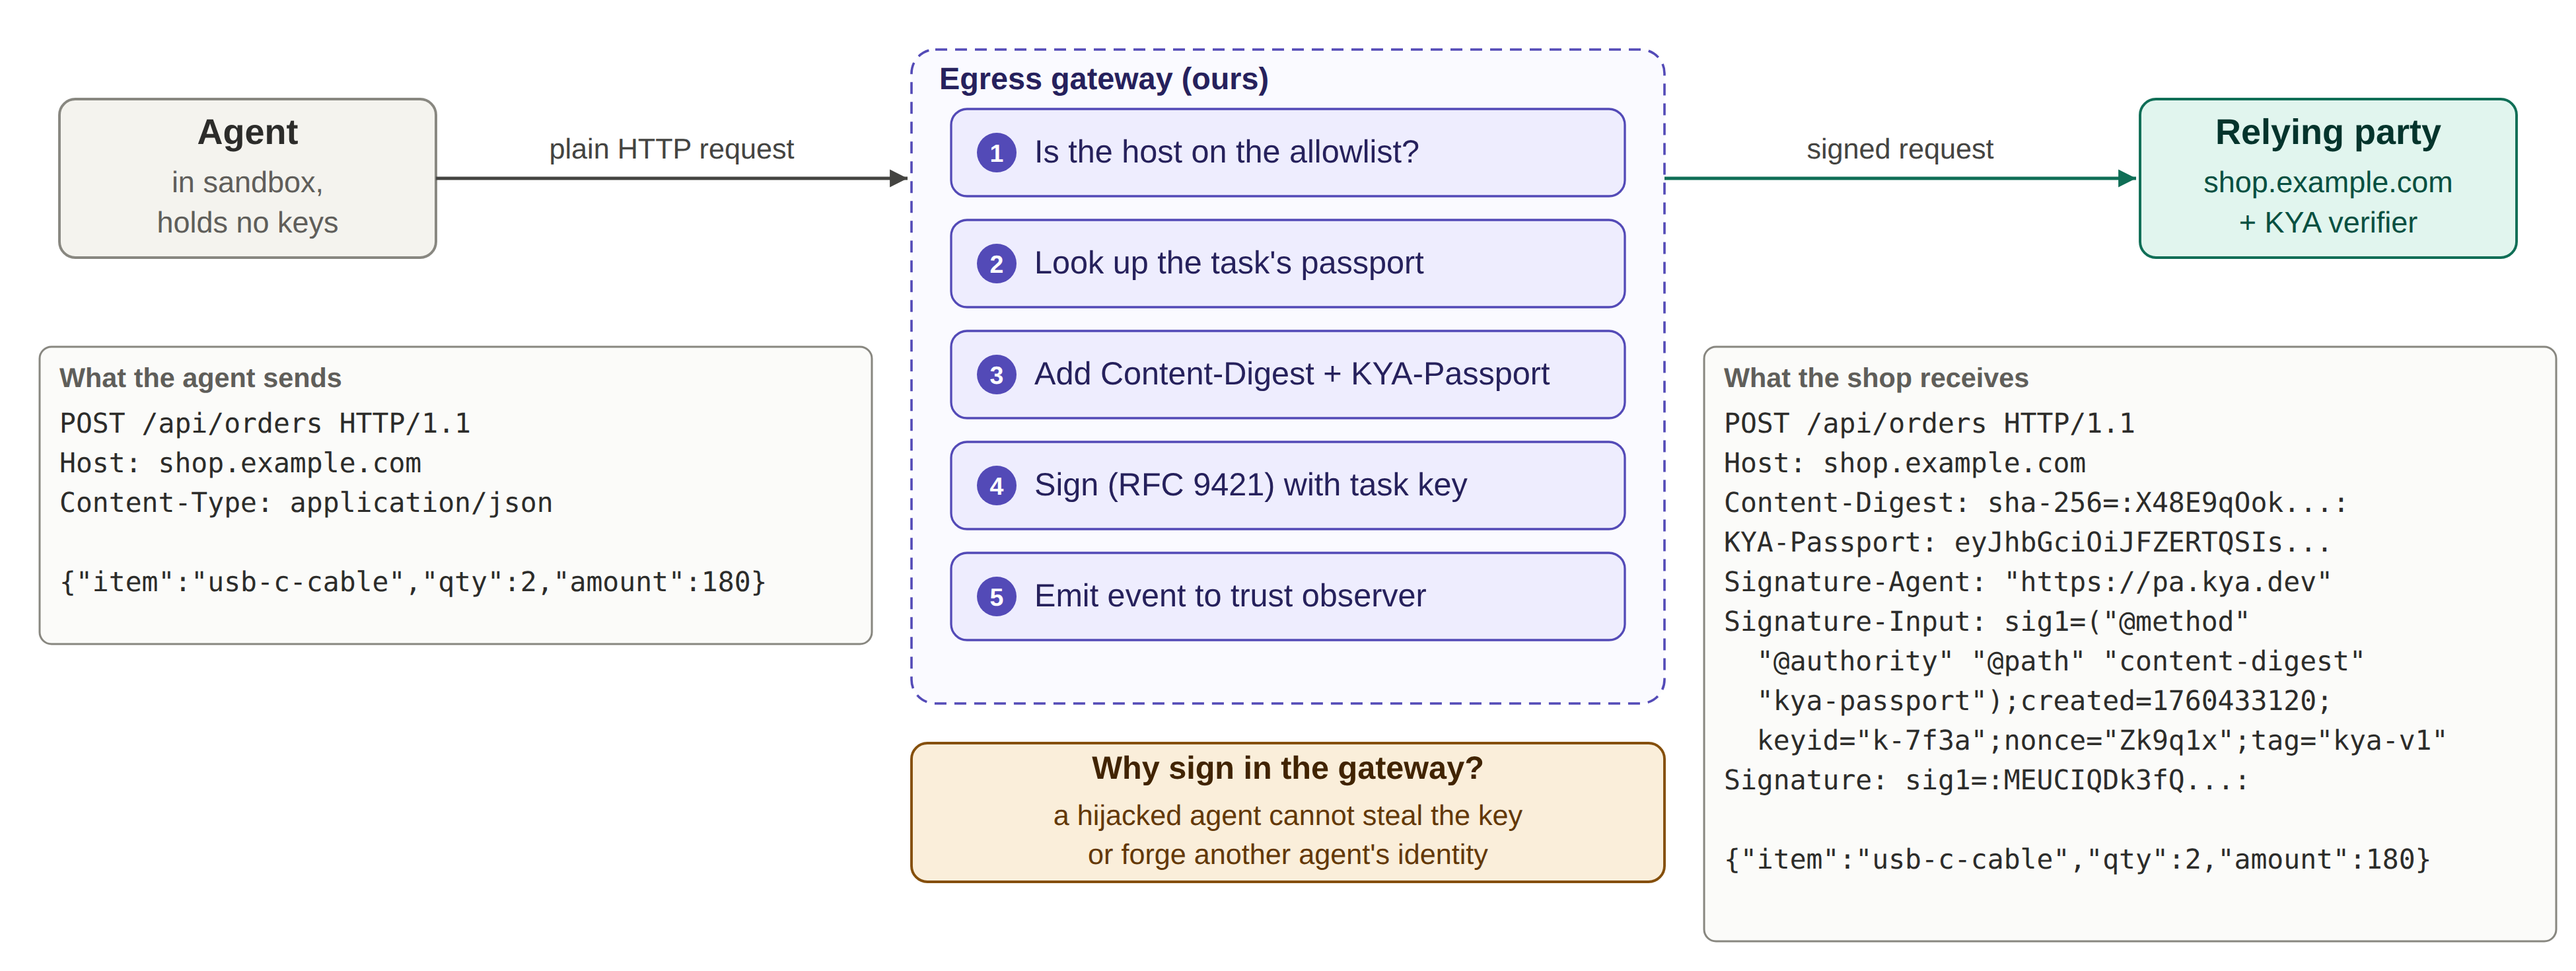
\includegraphics[width=\linewidth]{signing.png}
  \caption{The egress gateway turns a plain request from the agent into a signed, attributable request. The agent itself never sees the key.}
  \label{fig:signing}
\end{figure}

\subsubsection{Identifying the calling task}

Each task's proxy URL contains a random 256-bit proxy credential (\codeurl{http://task:<credential>@kya-gateway:3128}), created by the admission proxy and bound to exactly one task. The gateway maps it to the task, its passport and its key. The credential is only accepted at the gateway, which is not reachable from outside the cluster. Where Agent Substrate exposes the actor-to-worker mapping, the gateway additionally checks the source address.

\subsubsection{Seeing inside HTTPS}

To sign a request, the gateway must see its method, path, headers and body. For HTTPS this means the gateway terminates the agent's TLS connection with a certificate issued by the cluster-local gateway CA (installed by the KYA runner) and opens a new, normal TLS connection to the real destination. This is the same technique corporate proxies use. It makes the gateway a highly trusted component (Section~\ref{sec:threats}); in exchange, agents need no code changes at all. Agents that want to avoid interception can instead send plain HTTP to the gateway with an explicit target, and the gateway performs TLS upstream.

\subsubsection{The signature}

The gateway signs with HTTP Message Signatures (RFC~9421), following the Web Bot Auth profile~\cite{webbotauth} where possible:

\begin{itemize}
  \item covered components: \code{@method}, \code{@authority}, \code{@path}, \code{content-digest} (RFC~9530 hash of the body) and \code{kya-passport};
  \item parameters: \code{created} (Unix time), \code{keyid} (the task key id), a random \code{nonce}, and \code{tag="kya-v1"};
  \item a \code{Signature-Agent} header pointing to the PA, so that verifiers know where to find issuer keys.
\end{itemize}

Covering the passport header in the signature ties the passport to this specific request; covering the digest ties the body; \code{created} and \code{nonce} let the verifier reject replays.

\subsubsection{Metering and credential injection}

Because every byte passes through it, the gateway also counts requests per host, bytes, and (for recognised LLM APIs) tokens used, and reports them to the observer as spend signals. As a stretch goal, the gateway can \emph{inject} the model provider's API key into LLM calls, so that the key referenced by AX's \code{Model} resource no longer needs to be present inside the sandbox at all (NFR5).

%-----------------------------------------------------------------
\subsection{Verifier SDK}\label{sec:verifier}

\textbf{Responsibility:} let a relying party decide, for each incoming request, whether to serve it.

The verifier is a library with two initial bindings: a Spring Boot starter (servlet filter + annotations) and a Go \code{net/http} middleware. It follows the decision procedure in Figure~\ref{fig:verifier}. The checks are ordered from cheapest to most expensive, and each failure has its own, explicit response.

\begin{figure}[H]
  \centering
  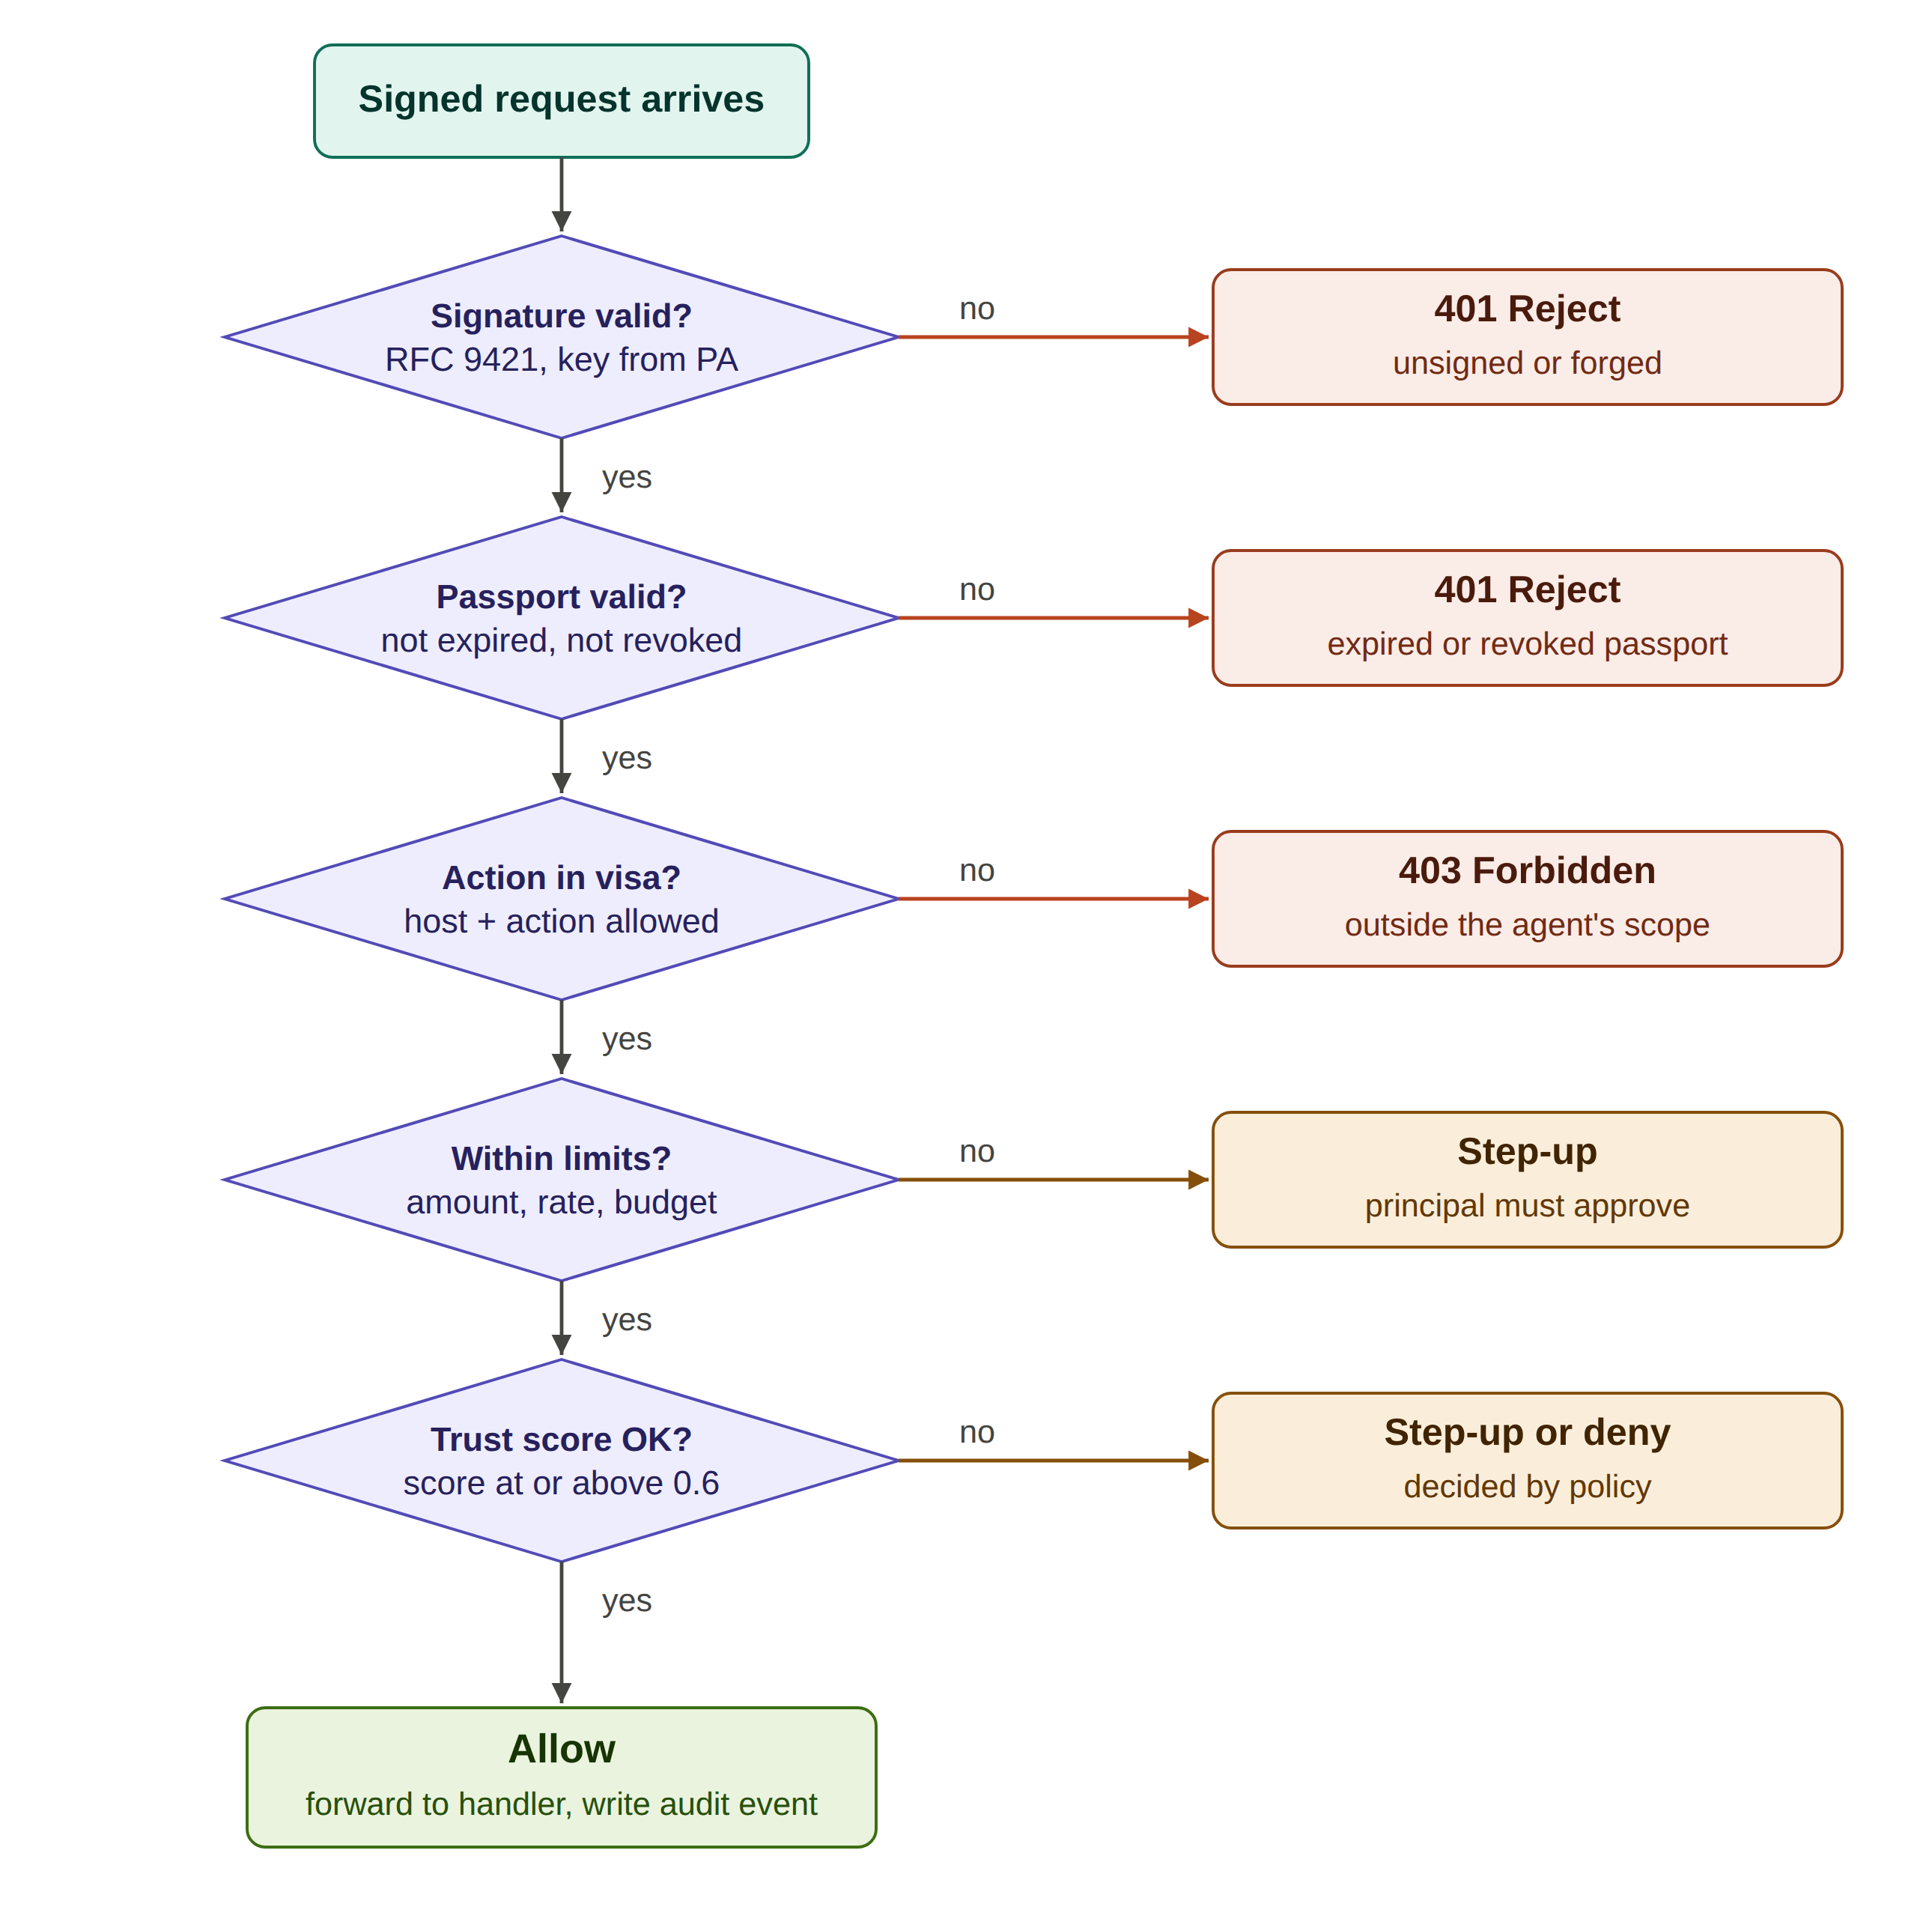
\includegraphics[width=0.78\linewidth]{verifier_flow.png}
  \caption{Decision procedure of the KYA verifier. Red outcomes are hard failures; amber outcomes ask the principal to approve.}
  \label{fig:verifier}
\end{figure}

Integration into an existing Spring Boot service is intentionally small:

\begin{lstlisting}[language=Java,caption={Protecting an endpoint with the Spring Boot binding (planned API).}]
// application.yml
// kya:
//   issuer: https://pa.kya.dev
//   audience: shop.example.com
//   revocation-refresh: 30s

@RestController
class OrderController {

  @PostMapping("/api/orders")
  @KyaAction(value = "order.create", amount = "#body.amount", currency = "TRY")
  ResponseEntity<Order> create(@RequestBody OrderRequest body, KyaContext kya) {
    log.info("order from agent {} on behalf of {}", kya.agentId(), kya.principal());
    return ResponseEntity.status(201).body(orders.create(body, kya.principal()));
  }
}
\end{lstlisting}

The \code{@KyaAction} annotation names the action and tells the verifier how to read the amount from the request. Requests \emph{without} any KYA headers (for example from human users in a browser) are passed through unchanged by default, so the verifier can be adopted gradually; a service can also choose \code{kya.mode=required} to accept only verified agents.

\subsubsection{Step-up approvals}\label{sec:stepup}

Some requests are valid but too risky to execute without a human: the amount exceeds the passport's \code{approval\_above}, the relying party has its own rule (for example ``orders above 1,000~TRY from agents need a human''), or the task's trust score is in the step-up band. The design follows three principles:

\begin{enumerate}
  \item \textbf{The relying party never contacts the human.} It usually does not even know who the principal is. It only says ``approval required'' and later verifies a signed proof. Contacting the principal is the job of the KYA platform, which authenticated that person at launch. The division of roles is the same as in 3-D Secure card payments: the shop does not send you an SMS, your bank does, and the shop only checks the bank's signed answer.
  \item \textbf{The agent is informed, not bypassed.} Human approval can take minutes. If the agent were kept in the dark (for example by the gateway silently holding the request), its HTTP client would time out, it would retry or look for another shop, and it could not tell its own user what is happening or adapt to a rejection. The agent therefore receives an explicit, machine-readable answer and can follow the approval's status.
  \item \textbf{The agent can see the approval, but never grant it.} Granting requires the principal's own OIDC login in the console. Everything exposed to the agent is read-only, and the grant is bound to one exact request.
\end{enumerate}

Figure~\ref{fig:stepup} shows the complete flow.

\begin{figure}[H]
  \centering
  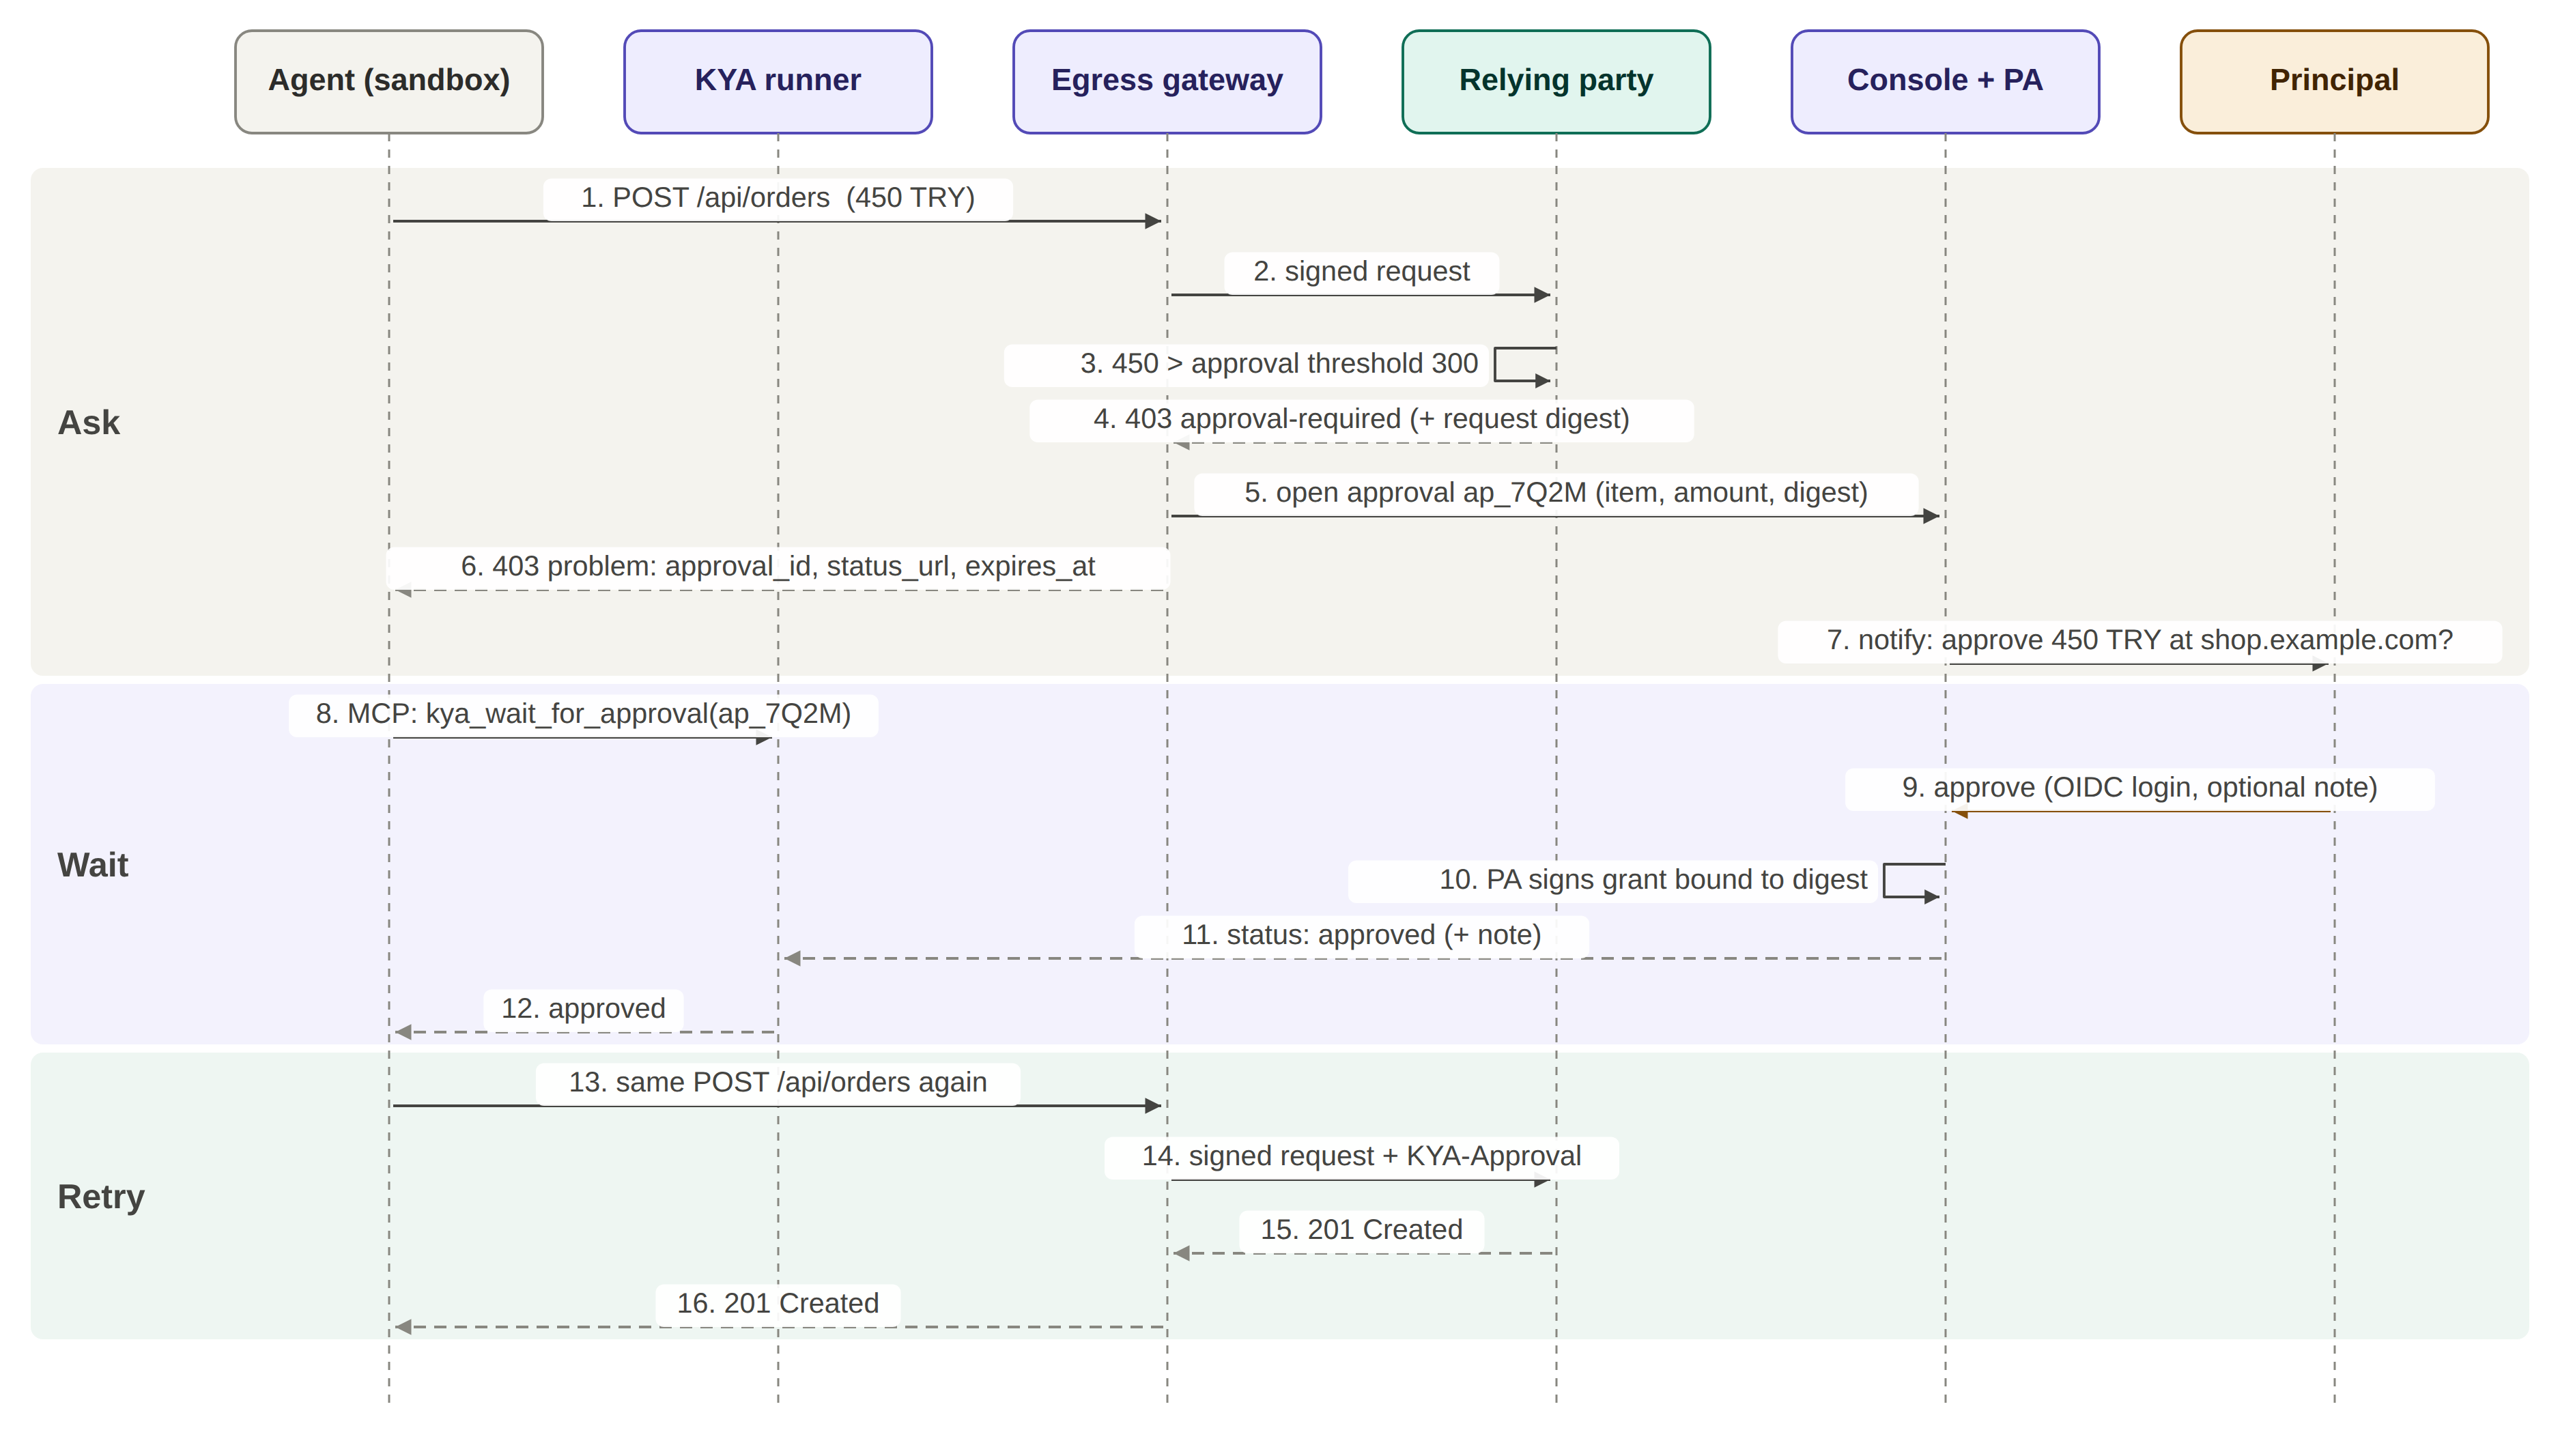
\includegraphics[width=\linewidth]{stepup.png}
  \caption{Agent-aware step-up approval. The agent receives an explicit ``approval required'' answer, waits through a read-only status channel, and repeats the same request once the principal has approved. Only the principal, logged in to the console, can approve.}
  \label{fig:stepup}
\end{figure}

\paragraph{1. The relying party asks for approval.} Instead of processing the request, the verifier answers with an RFC~9457 problem document containing the digest of the request it refused:

\begin{lstlisting}[language=json]
HTTP/1.1 403 Forbidden
Content-Type: application/problem+json

{
  "type": "https://kya.dev/problems/approval-required",
  "title": "Principal approval required",
  "reason": "amount 450 TRY exceeds approval threshold 300 TRY",
  "request_digest": "sha-256=:q1Xk...:"
}
\end{lstlisting}

\paragraph{2. The gateway opens an approval and tells the agent.} The gateway recognises this response type, creates approval \code{ap\_7Q2M} in the console (with the relying party's host, the parsed item and amount, and the request digest), and passes the answer on to the agent, enriched with what the agent needs to follow up:

\begin{lstlisting}[language=json]
HTTP/1.1 403 Forbidden
Content-Type: application/problem+json
Retry-After: 30

{
  "type": "https://kya.dev/problems/approval-required",
  "title": "Principal approval required",
  "reason": "amount 450 TRY exceeds approval threshold 300 TRY",
  "approval_id": "ap_7Q2M",
  "status_url": "http://127.0.0.1/kya/v1/approvals/ap_7Q2M",
  "expires_at": "2026-10-14T09:31:00Z"
}
\end{lstlisting}

Any agent that reads HTTP responses can understand this; no framework-specific integration is required.

\paragraph{3. The agent follows the status.} The \code{status\_url} points to the KYA runner inside the sandbox, so it never leaves the sandbox and is not subject to the host allowlist. It returns \code{pending}, \code{approved}, \code{rejected} or \code{expired}, and, if the principal wrote one, a note. The runner obtains the status from the console through a read-only, task-scoped call. For agents that use tools, the runner also registers an MCP server in the task's workspace with three tools:

\begin{center}
\small
\begin{tabularx}{\linewidth}{@{}L{5.4cm}Y@{}}
\toprule
\textbf{MCP tool} & \textbf{Purpose}\\
\midrule
\code{kya\_my\_permissions()} & Returns the effective visa: hosts, actions, limits and approval thresholds. Lets the agent know \emph{before} checkout that a 450~TRY order will need approval.\\
\code{kya\_approval\_status(id)} & Current status of an approval, with the principal's note if any.\\
\code{kya\_wait\_for\_approval(id, timeout)} & Blocks until the approval is decided or the timeout passes.\\
\bottomrule
\end{tabularx}
\end{center}

While waiting, the agent can tell its own user what it is waiting for, or continue with other parts of its task.

\paragraph{4. The principal decides.} The console notifies the principal (web push or e-mail in the prototype). The approval page shows two clearly separated kinds of information: \emph{verified facts} taken from the refused request and the relying party (host, item, amount), and the agent's own \emph{justification}, if it supplied one, labelled as an unverified claim. The distinction matters because the agent's text may itself be the product of a prompt injection. The principal approves or rejects and may add a note (``the 4-port model is enough'').

\paragraph{5. The agent acts on the decision.} If approved, the PA issues a short-lived \textbf{approval grant} (five minutes), a signed token bound to the exact request digest, similar in spirit to the user-signed ``mandates'' of the Agent Payments Protocol~\cite{ap2}. The agent sends \emph{the same request again}; the gateway finds a grant whose digest matches, attaches it in a \code{KYA-Approval} header, and the verifier accepts the request after checking the grant's signature and digest. If the agent changes anything (item, quantity, amount), the digest no longer matches and a new approval is needed. If rejected, the agent receives the rejection and the note, and can adapt its plan.

\paragraph{Interaction with the trust observer.} An \code{approval-required} answer is not a violation: the agent is doing exactly what the rules ask. It therefore carries no trust penalty. Only abuse of the mechanism is penalised, for example opening many approvals for slightly different requests in a short time, which would amount to spamming the principal.

%-----------------------------------------------------------------
\subsection{Trust observer}

\textbf{Responsibility:} continuously estimate how much each running task should be trusted, and act when trust drops.

Figure~\ref{fig:observer} shows the pipeline from raw signals to actions.

\begin{figure}[H]
  \centering
  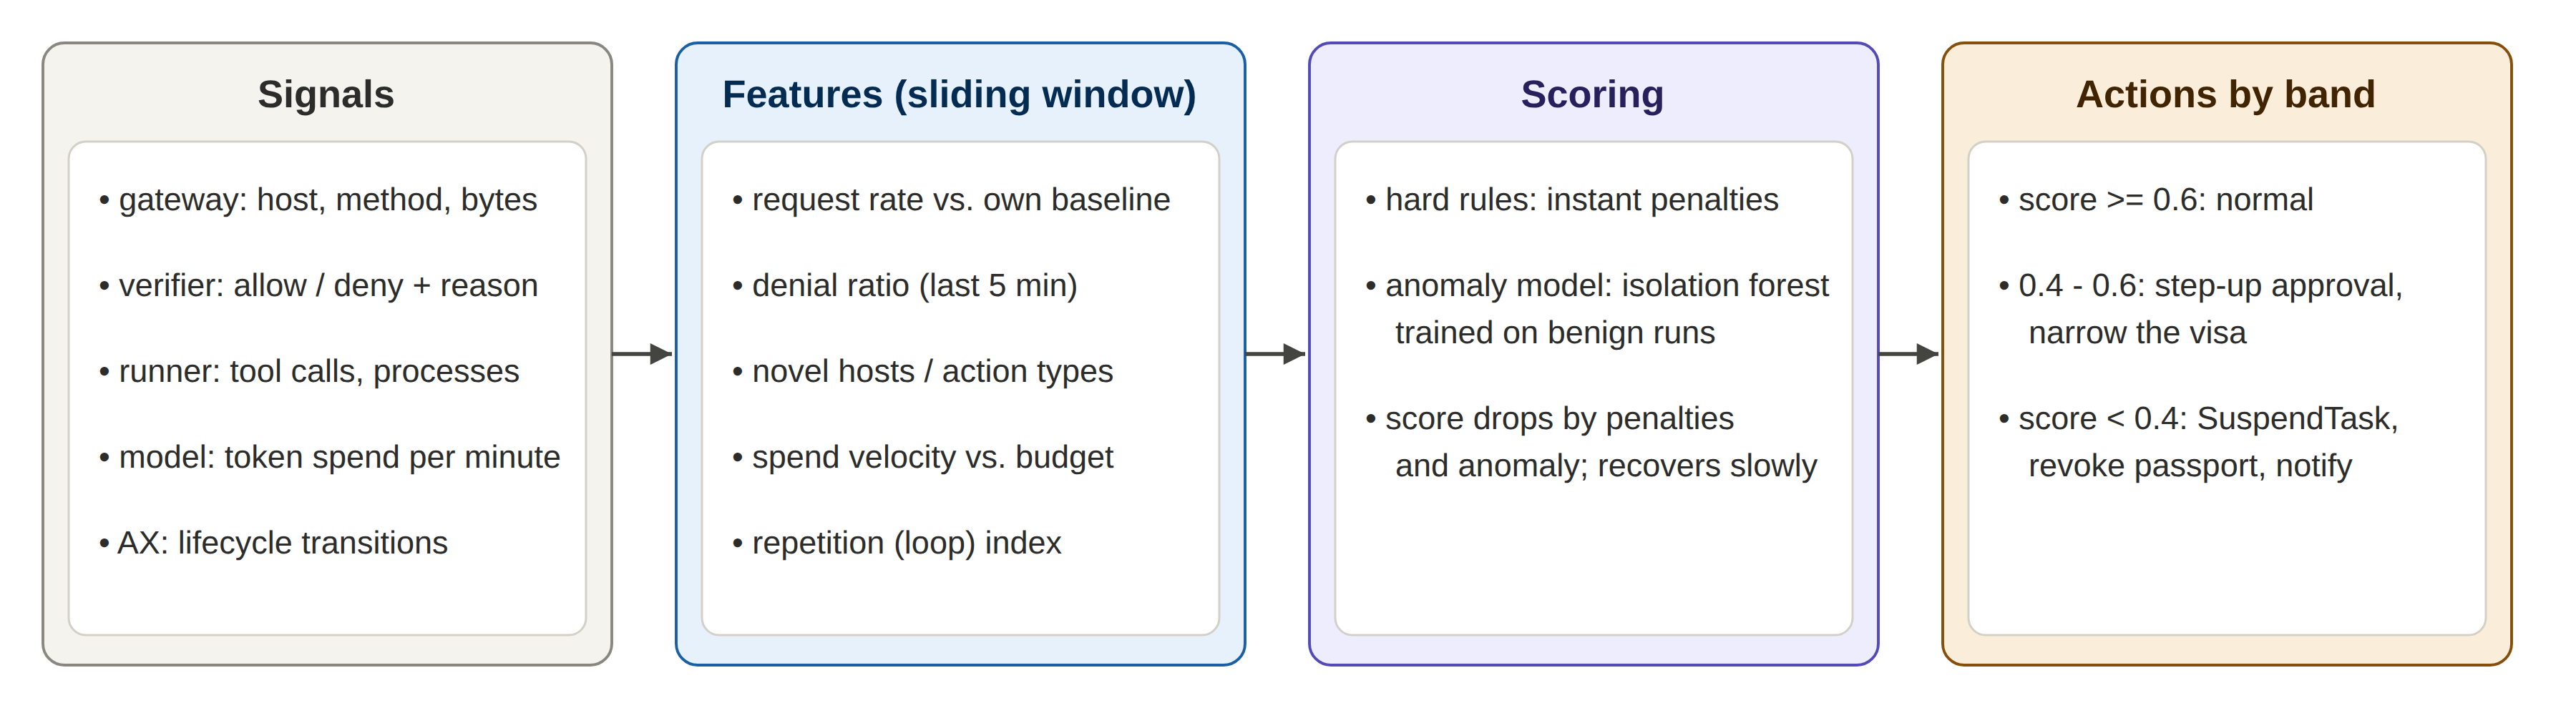
\includegraphics[width=\linewidth]{observer.png}
  \caption{Trust observer pipeline: signals from all components become per-task features, which are scored and mapped to actions.}
  \label{fig:observer}
\end{figure}

\subsubsection{Signals and features}

Signals arrive as events (JSON over a message queue; OpenTelemetry-compatible attributes). For each task, the observer maintains sliding-window features, including: request rate relative to the task's own recent baseline, ratio of denied requests, number of never-before-seen hosts and action types for this image, spend velocity relative to the remaining budget, and a repetition index (how often the last $k$ requests repeat the same method, path and body hash, which detects loops).

\subsubsection{Score}

Each task starts with score $s_0 = 0.8$. At every event the score is updated as
\[
  s_t \;=\; \operatorname{clip}_{[0,1]}\!\Big( s_{t-1} \;+\; \lambda\,(s_0 - s_{t-1}) \;-\; \sum_i p_i(t) \;-\; \beta \cdot \max\big(0,\; a_t - \tau\big) \Big),
\]
where:
\begin{itemize}
  \item $p_i(t)$ are \textbf{rule penalties} for hard signals in this event (for example: egress denied $0.15$; verifier \code{403} for an out-of-scope request $0.20$; new action type $0.10$; budget more than 80\% used $0.10$; \code{approval-required} answers carry no penalty, see Section~\ref{sec:stepup});
  \item $a_t \in [0,1]$ is the \textbf{anomaly score} of the current feature vector, produced by an isolation forest~\cite{iforest} trained on benign runs of the same agent image, and $\tau$ its tolerance;
  \item $\lambda$ is a small \textbf{recovery rate}: trust returns slowly towards $s_0$ when nothing bad happens, so a single false alarm does not permanently cripple a task.
\end{itemize}

Rules make the observer predictable and explainable (every penalty appears in the audit ledger with its reason); the anomaly model catches patterns nobody wrote a rule for. Tuning $\lambda$, $\beta$, $\tau$ and the penalties is part of the evaluation (Section~\ref{sec:eval}).

\subsubsection{Actions}

\begin{center}
\small
\begin{tabularx}{\linewidth}{@{}L{3cm}Y@{}}
\toprule
\textbf{Score band} & \textbf{Action}\\
\midrule
$s \ge 0.6$ & Normal operation.\\
$0.4 \le s < 0.6$ & Step-up: every state-changing request needs principal approval; the PA may issue a narrower replacement passport (for example, read-only actions).\\
$s < 0.4$ & Call \code{SuspendTask} on AX, revoke the passport, notify the principal. The suspended task keeps its memory and workspace, so an operator can inspect it (\code{ax ssh}) and resume it if it was a false alarm.\\
\bottomrule
\end{tabularx}
\end{center}

Figure~\ref{fig:trust} shows the score of a task that behaves normally for twelve minutes and is then hijacked (the full story is Example~2 in Section~\ref{sec:ex-injection}).

\begin{figure}[H]
  \centering
  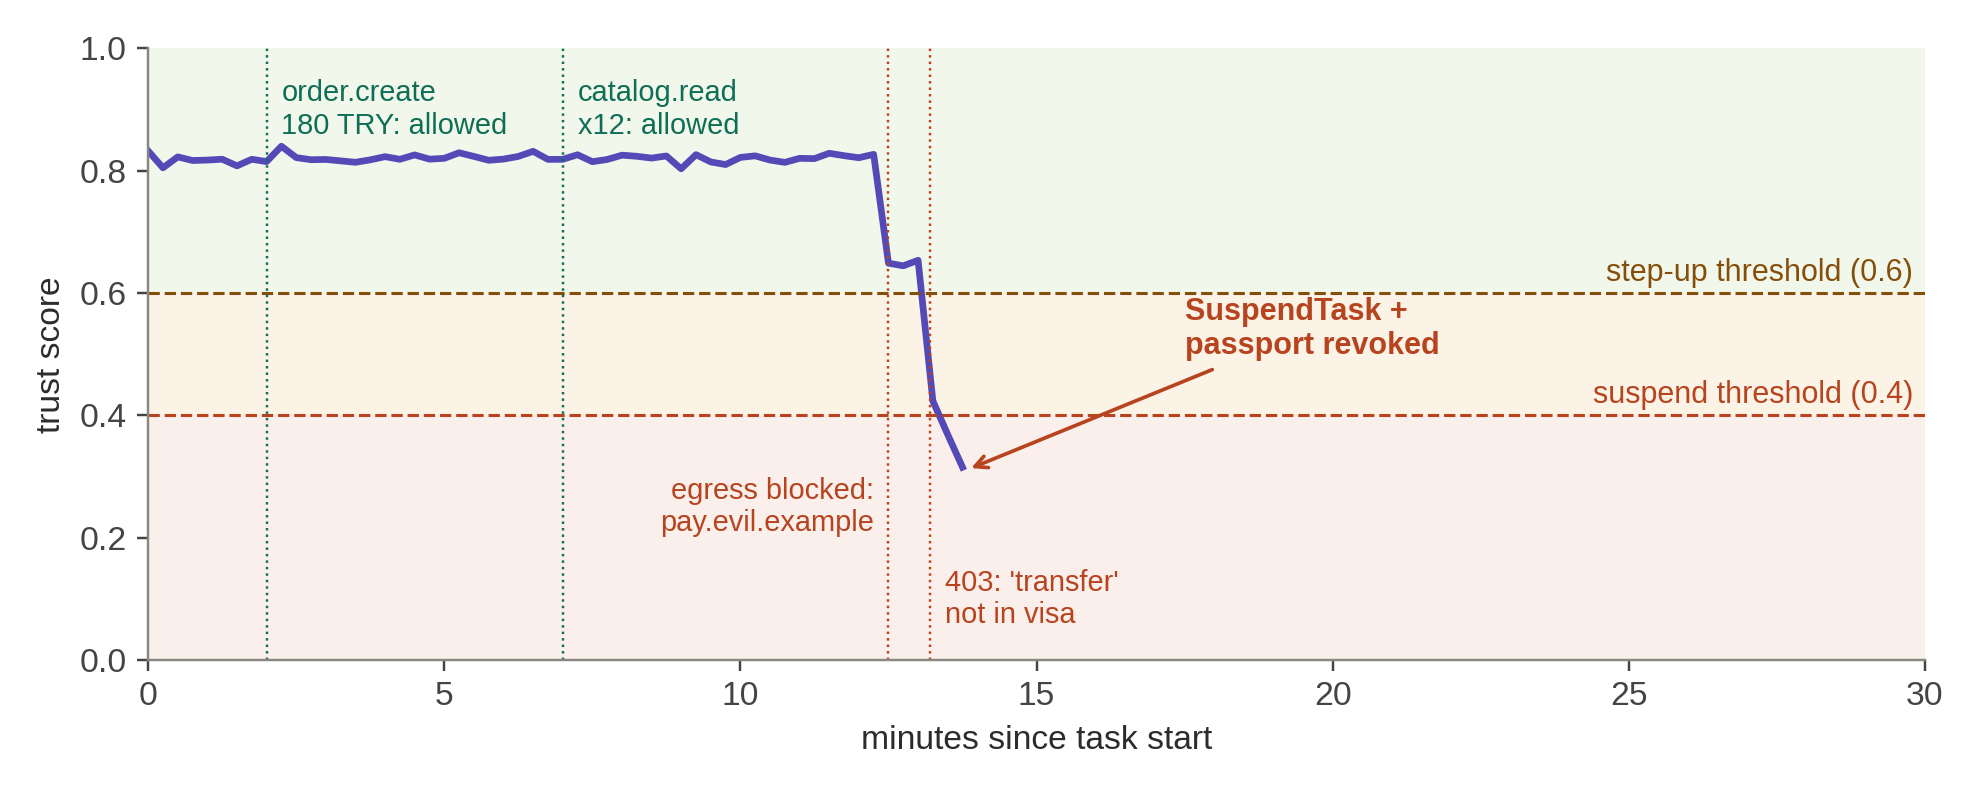
\includegraphics[width=0.95\linewidth]{trust_score.png}
  \caption{Trust score over time. Normal activity keeps the score around 0.82. Two denied requests and a never-seen action type within 40 seconds push it below the suspend threshold, and the observer suspends the task.}
  \label{fig:trust}
\end{figure}

%-----------------------------------------------------------------
\subsection{Delegation chains}\label{sec:delegation}

AX expects agents to break work into trees of tasks~\cite{ax-concepts}. Without care, a sub-task could end up with more power than its parent. AgentPassport enforces \textbf{attenuation}: a child's visa is always a subset of its parent's, and its limits are carved out of the parent's budget (Figure~\ref{fig:delegation}).

\begin{figure}[H]
  \centering
  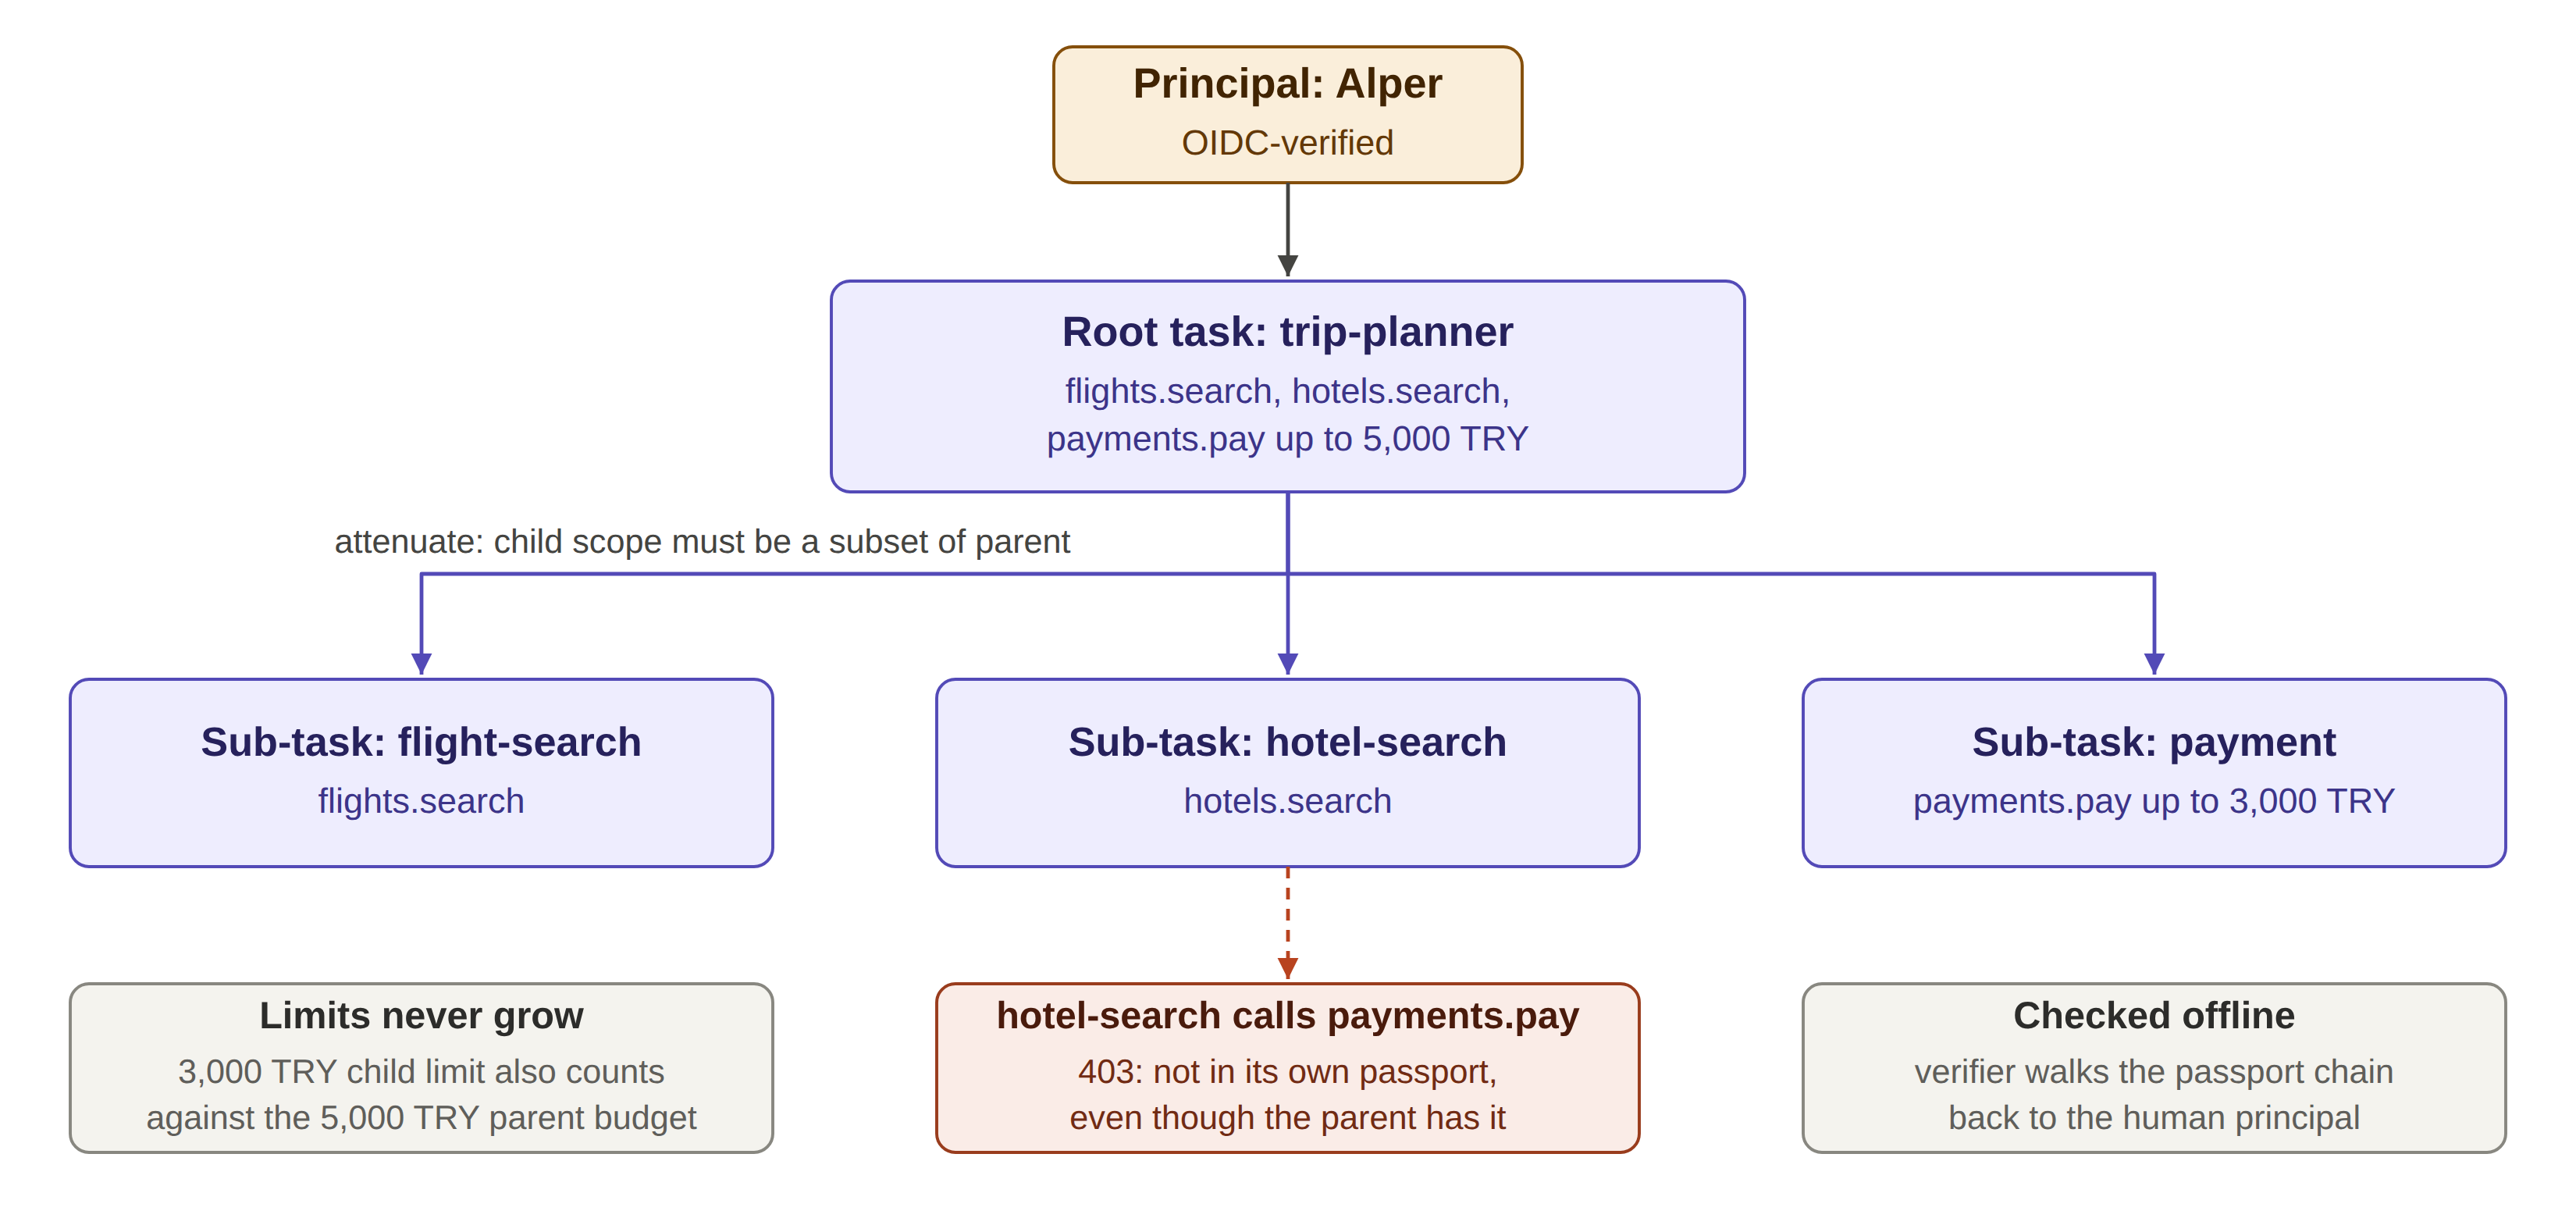
\includegraphics[width=\linewidth]{delegation.png}
  \caption{Delegation with attenuation. Each sub-task receives only the permissions it needs; a sub-task that tries to use a permission of its parent is rejected.}
  \label{fig:delegation}
\end{figure}

When an agent creates a sub-task, its \code{CreateTask} call also goes through the admission proxy (the only path to \code{ax-server}), authenticated by the parent's proxy credential. The proxy calls \code{:delegate} on the PA, which checks that
\begin{itemize}
  \item the requested hosts and actions are a subset of the parent's;
  \item every limit is at most the parent's remaining budget, which is then reserved;
  \item the delegation depth does not exceed \code{maxDelegationDepth};
  \item the child's expiry is not later than the parent's.
\end{itemize}

The child passport's \code{parent} claim contains the parent's \code{jti}, and its principal block is copied from the parent, so the chain always ends at a human. Verifiers can walk the chain (each link is a passport signed by the PA) and re-check the subset relation as defence in depth. Revoking a parent revokes all its descendants. As a research extension, we will compare this PA-mediated approach with Biscuit tokens~\cite{biscuit}, which allow attenuation offline without contacting the PA.

%-----------------------------------------------------------------
\subsection{Audit ledger}

\textbf{Responsibility:} keep a complete, tamper-evident history of security-relevant events.

The ledger is an append-only table in PostgreSQL. Each entry contains its sequence number, timestamp, event type, subject (task, passport, principal), details, and two hashes: the hash of the previous entry and its own hash, computed as $h_n = \mathrm{SHA\text{-}256}(h_{n-1} \,\|\, \mathrm{canonical}(e_n))$ (Figure~\ref{fig:audit}). Changing or deleting any past entry changes every later hash. Every five minutes the PA signs a \emph{checkpoint} (latest sequence number and hash) and publishes it, so that even the database administrator cannot silently rewrite history.

\begin{figure}[H]
  \centering
  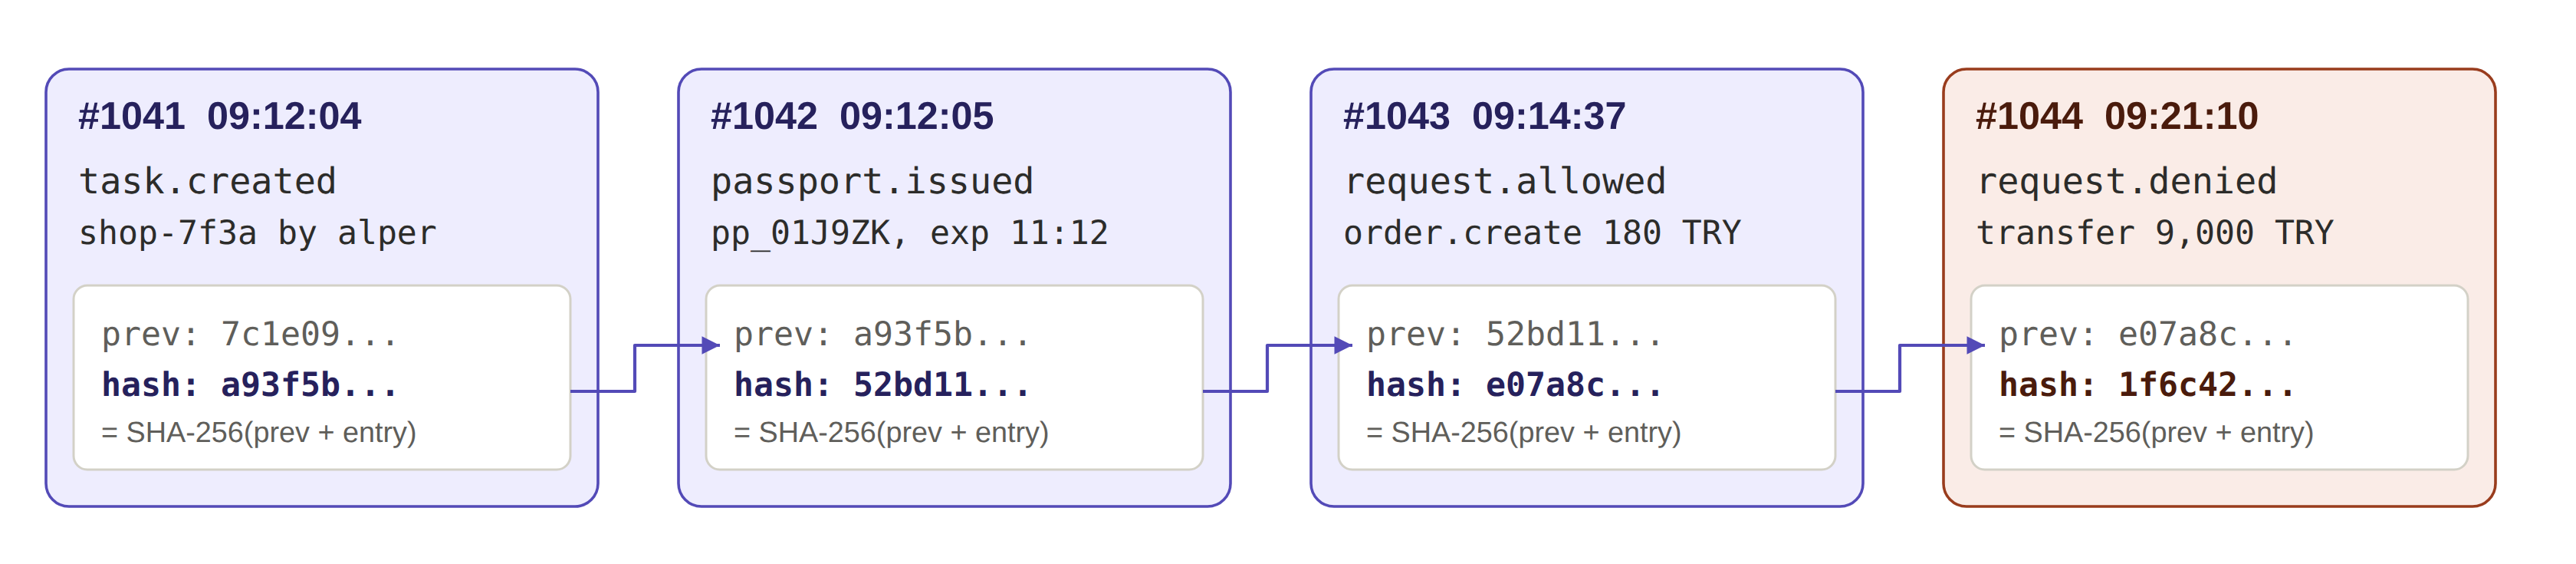
\includegraphics[width=\linewidth]{audit_chain.png}
  \caption{Hash-chained audit entries for the task in the examples. Each entry commits to all entries before it.}
  \label{fig:audit}
\end{figure}

{\raggedright Events recorded include \code{task.created}, \code{task.rejected}, \code{passport.issued}, \code{passport.revoked}, \code{egress.denied}, \code{request.allowed}, \code{request.denied}, \code{approval.requested}, \code{approval.granted}, \code{trust.changed} and \code{task.suspended}.\par}

%-----------------------------------------------------------------
\subsection{Console}

The console is a web application (React front end, served by a small backend that reads the ledger, the PA and the observer). It offers:
\begin{itemize}
  \item \textbf{My agents}: the principal's running tasks, with passport, visa, remaining budget and live trust score;
  \item \textbf{Approvals}: pending step-up requests with the full request, approve/reject buttons;
  \item \textbf{Incidents}: denied requests and suspensions, with the events that caused them;
  \item \textbf{Audit explorer}: search the ledger and verify the hash chain in the browser;
  \item \textbf{Operator views}: policies, fleet-wide statistics, revocation controls.
\end{itemize}
